\documentclass[english,10pt,a4paper]{article}
\usepackage[T1]{fontenc}
\usepackage{babel}
\usepackage{graphicx}
\usepackage{comment}
\title{Multivariate Statistical Techniques Assignment 2 2024}
\author{Mashiane Tshepiso 22692037}

\begin{document}
	\maketitle
	\section*{Question 1}
	\subsection*{a.}
	
		
	\begin{figure}[h]
	
		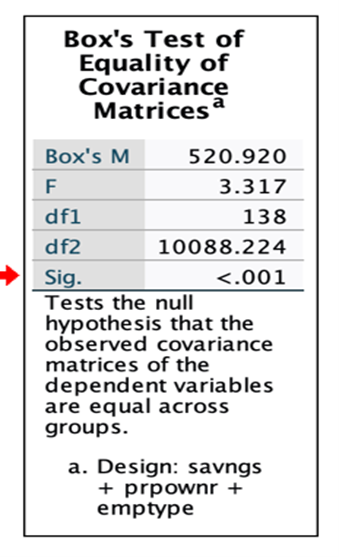
\includegraphics[width=0.2\linewidth]{Box's test2} 
		
	\end{figure}
		
	\begin{figure}[h]
		
		
		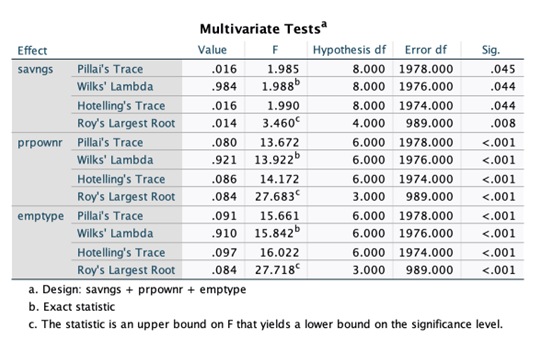
\includegraphics[width=1\linewidth]{Multivariate testQ1}
	\end{figure}
	
	
		\begin{figure}[h]
		
		
		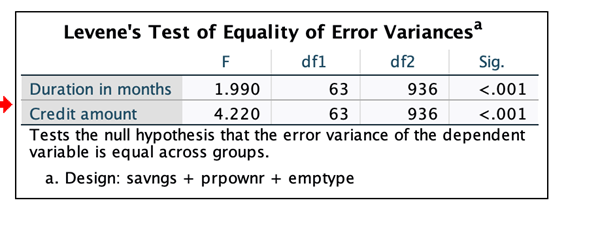
\includegraphics[width=1.5\linewidth]{Levene's testQ1}
		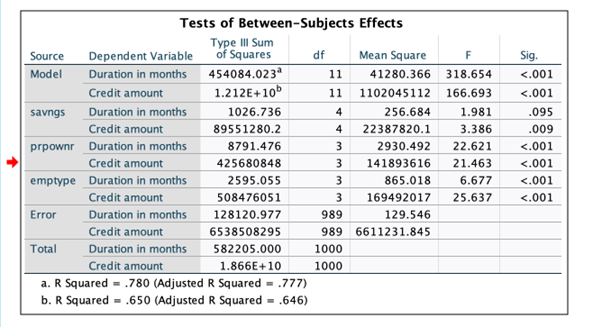
\includegraphics[width=1.5\linewidth]{Test between subject effectQ1}
	\end{figure}
	
	\begin{figure}[h]
		
		
		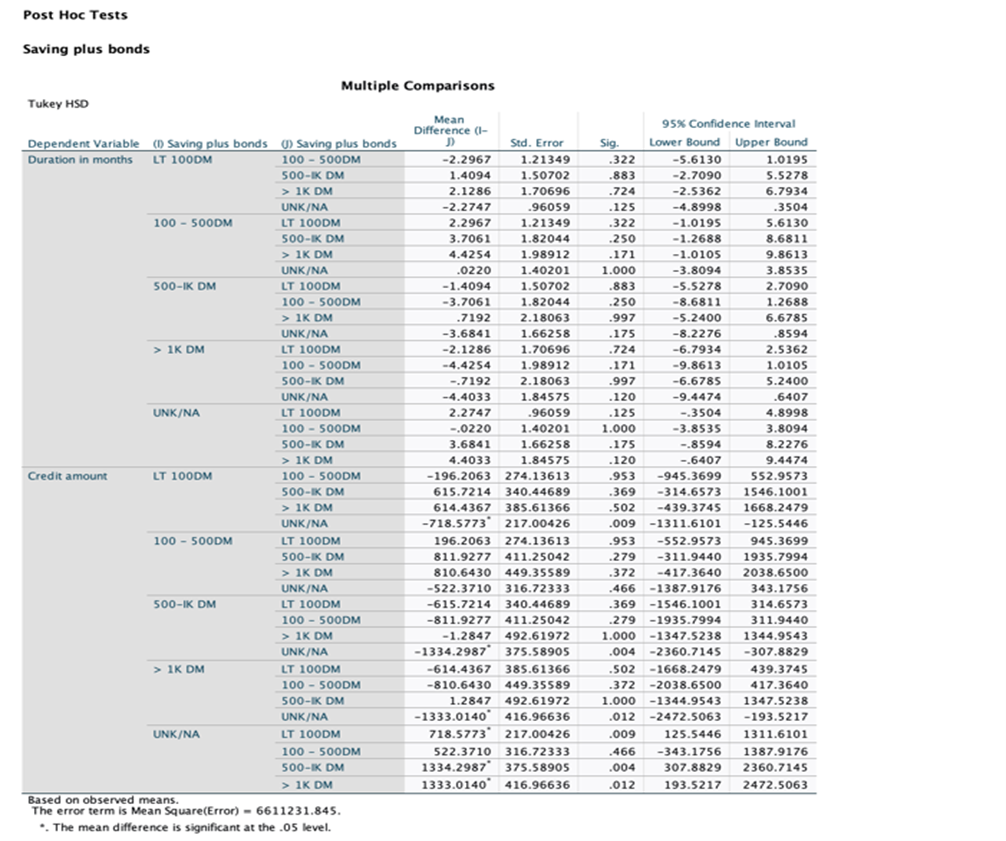
\includegraphics[width=2\linewidth]{Multiple comparison(savings plus bonus)}
	\end{figure}
	
	\begin{figure}[h]
		
		
		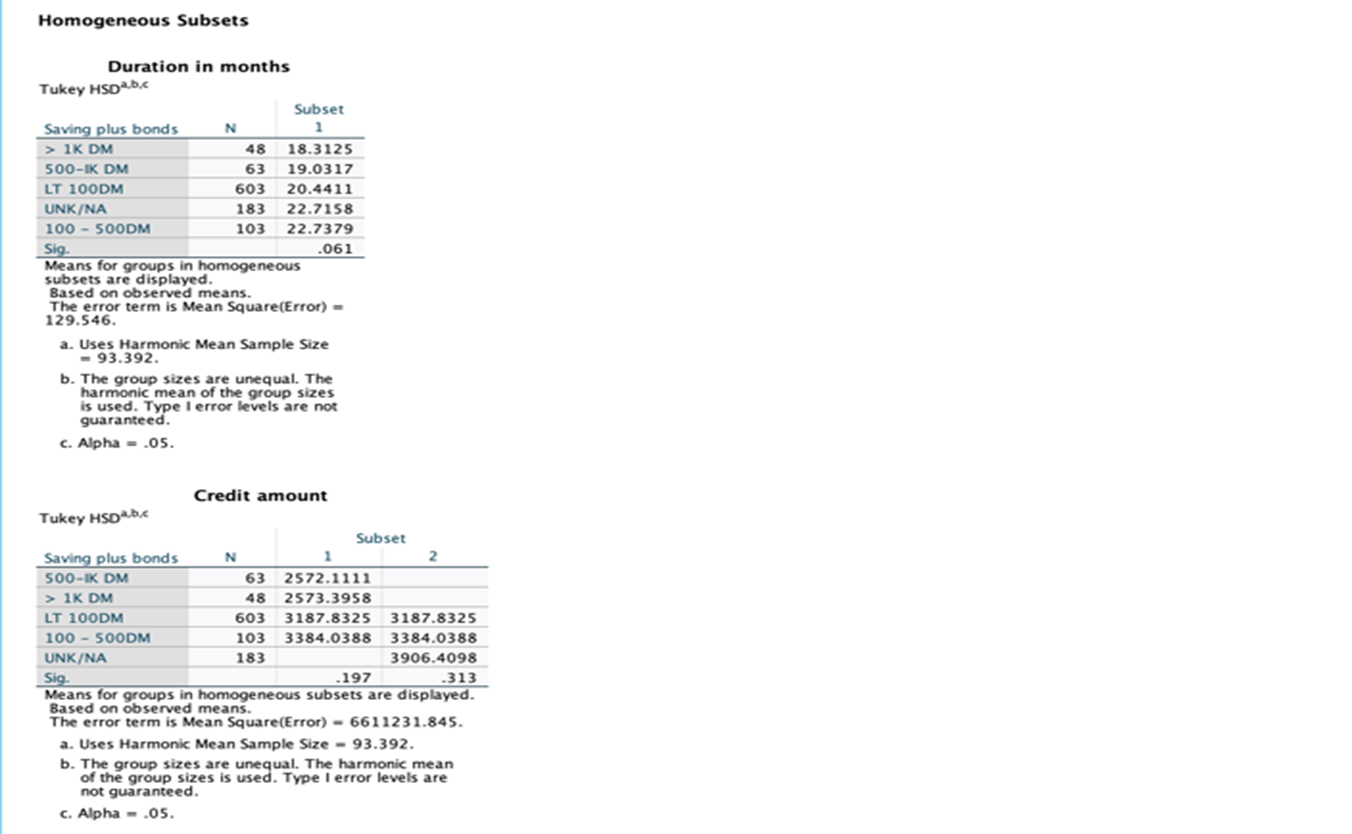
\includegraphics[width=1.2\linewidth]{post hoc test(saving plus bond)}
	\end{figure}
	
	
	\begin{figure}[h]
		
		
		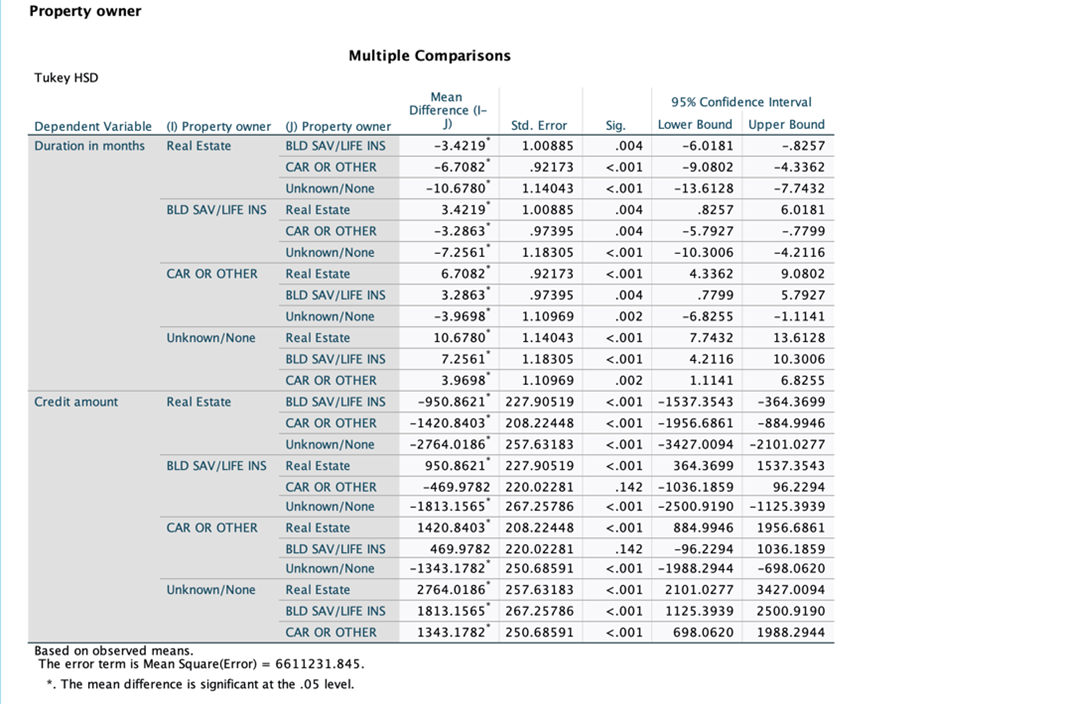
\includegraphics[width=1.2\linewidth]{Multiple comparison(property owner)}
	\end{figure}
	
	\begin{figure}[h]
		
		
		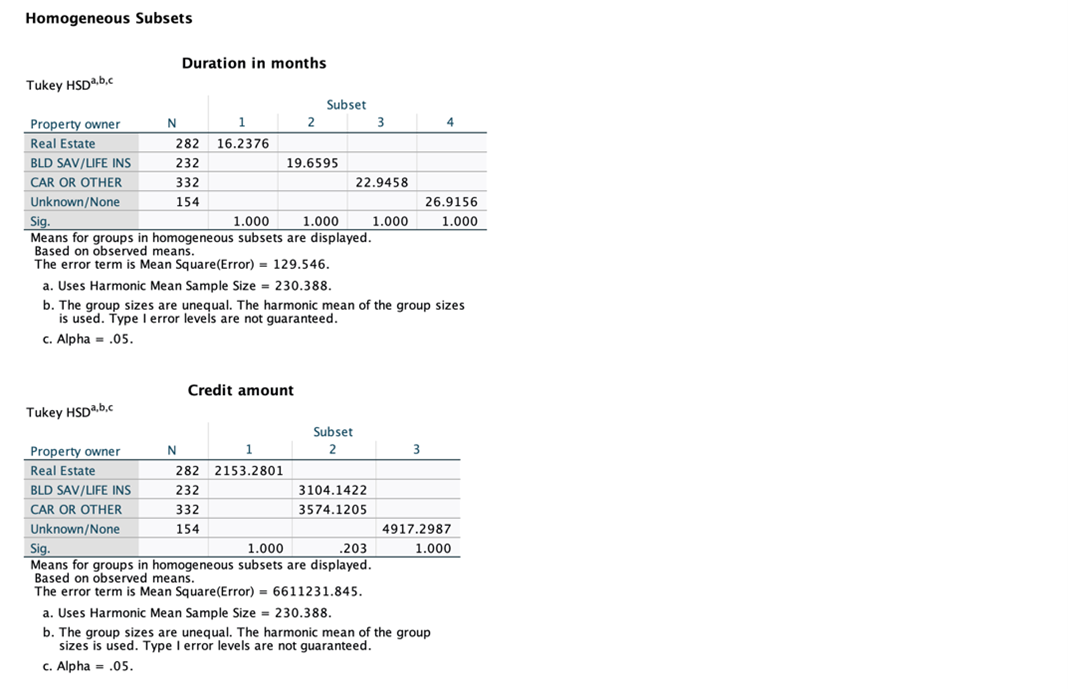
\includegraphics[width=1.2\linewidth]{post hoc test(property owner)}
	\end{figure}
	
	\begin{figure}[h]
		
		
		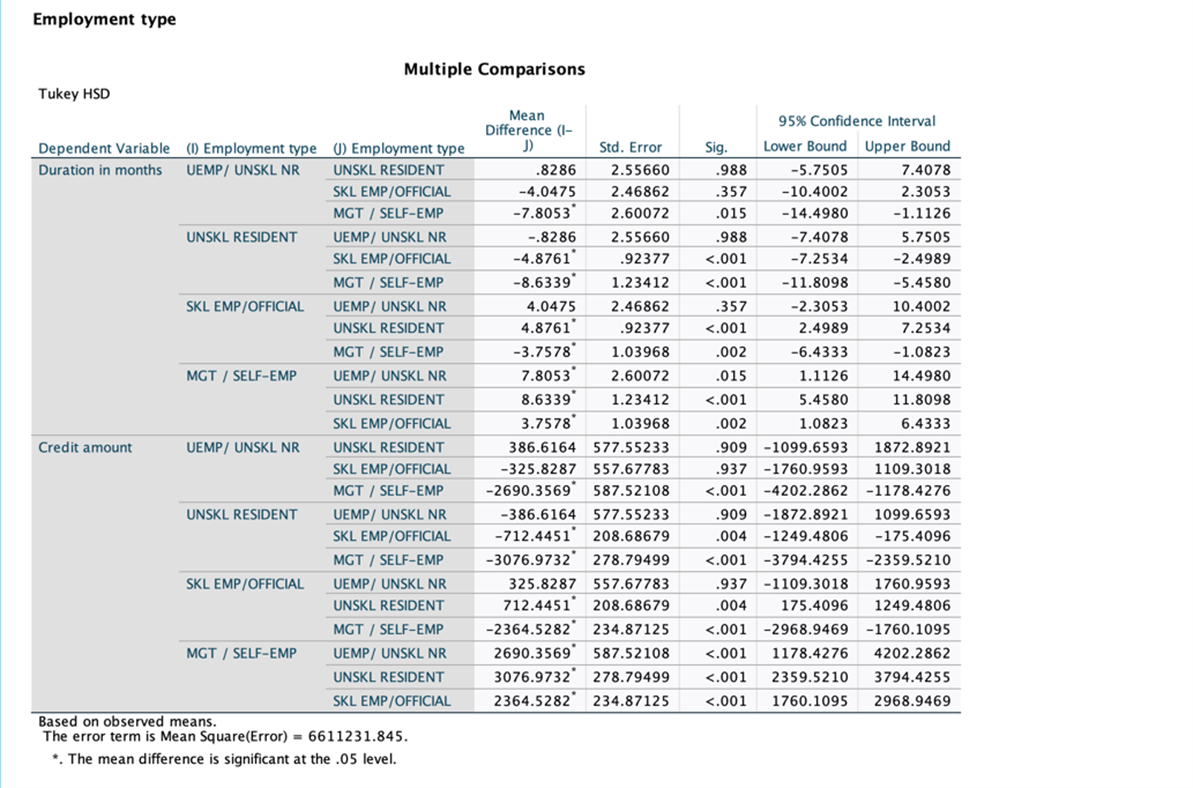
\includegraphics[width=1.2\linewidth]{Multiple comparison(emp type)}
	\end{figure}
	\begin{figure}[h]
		
		
		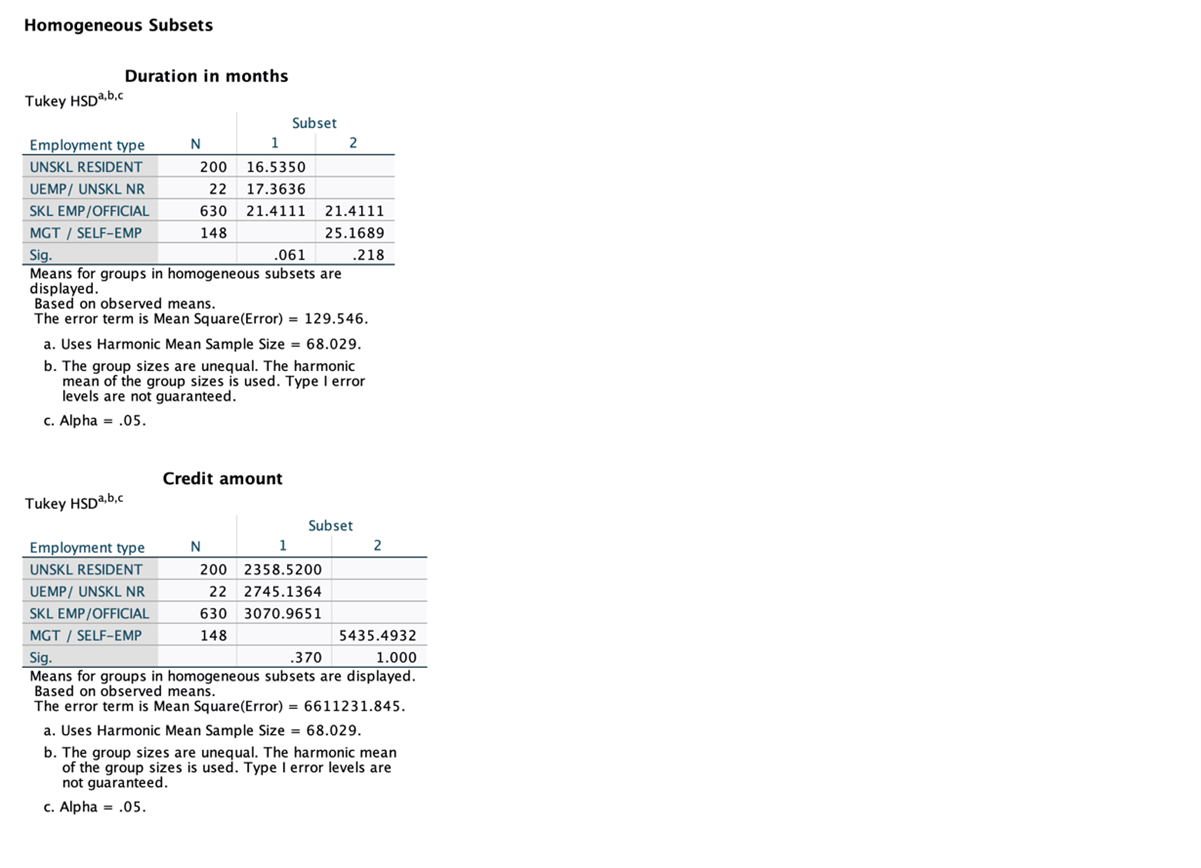
\includegraphics[width=1.2\linewidth]{post hoc test(emp type)}
	\end{figure}
	
%-------------------------------------------------------------
\begin{figure}[h]
	\subsection*{b. Interpretations}
	\subsubsection*{Box's test}	
	Since the associated p-value for the Box’s M Test is <0.001, which is less than the desired significance level of 0.05, this suggests that homogeneity of covariances is not met
	
	\subsubsection*{Multivariate Tests:}
For the "savings plus bond" effect, the Pillai's Trace statistic is 0.016, the F-statistic is 1.985, and the p-value is 0.045. This indicates that the "savings plus bond" effect is statistically significant at the 5\% Sig.level.

For the "property owner" effect, the Pillai's Trace statistic is 0.080, the F-statistic is 13.672, and the p-value is less than 0.001. This indicates that the "property owner" effect is statistically significant at the 5\% Sig.level.

For the "employment type" effect, the Pillai's Trace statistic is 0.091, the F-statistic is 15.661, and the p-value is less than 0.001. This indicates that the "employment type" effect is statistically significant at the 5\% Sig.level.

	\subsubsection*{Levene's Test of Equality of Error Variances.}
	For the "Duration in months" variable, the F-statistic is 1.990 with 63 and 936 degrees of freedom, and the p-value is less than 0.001.
	For the "Credit amount" variable, the F-statistic is 4.220 with 63 and 936 degrees of freedom, and the p-value is less than 0.001.
	The low p-values (less than 0.05) for both variables indicate that the we reject the null hypothesis of equal error variances across groups and conclude that the error variances are not equal across the groups defined by the independent variables("Duration"
	and "Credit amount").
	
		\subsubsection*{Tests between subjects effects:}
For the "Duration in months" dependent variable the p-values (Sig. column) for the Model, savings, property owner, and employment type effects are all less than 0.001, indicating that these effects are statistically significant at the 0.05 level of significance

For the "Credit amount" dependent variable the p-values (Sig. column) for the Model, savings, property owner, and employment type effects are all less than 0.001, indicating that these effects are statistically significant at the 0.05 level of significance

The low p-values (less than 0.05) for the majority of the effects suggest that the independent variables("savings", "property owner", and "employment type") ncluded in the model  have a significant impact on both dependent variables ("Duration in months" and "Credit amount").

\subsubsection*{Post Hoc Test: Saving Plus Bond}
	\subsubsection*{a.Multiple comparison:saving plus bond}
	
	For the "Duration in months" dependent variable the mean differences between various groups of "Saving plus bonds" are statistically insignificant, as indicated by the  p-values>0.05 (Sig. column).The 95\% confidence intervals for the mean differences include zero, further confirming the statistical insignificance of the differences.
	
	
	However for the "Credit amount" dependent variable to the "Duration in months" variable, the mean differences between various groups of "Saving plus bonds" are statistically significant, as indicated by the low p-values. And some of the 95\% confidence intervals for the mean differences do not include zero, further confirming the statistical significance of the differences.
	
	
\end{figure}

\begin{figure}[h]	
		\subsubsection*{b.Homogenious subset/duration in months: saving plus bonds}
		The group "> 1K DM" has a mean "Duration in months" of 18.3125, which is significantly different from the other groups.
		The groups "500-1K DM", "LT 100DM", and "UNK/NA" form a homogeneous subset, meaning they are not significantly different from each other.
		The group "100 - 500DM" has a mean "Duration in months" of 22.7379, which is significantly different from the other groups.
		
		
			\subsubsection*{c.Homogenious subset/credit amount:  saving plus bonds}
		
		The group "> 1K DM" and the group "500-1K DM" form Subset 1, with a mean "Credit amount" of 2572.1111 and 2573.3958, respectively.
		The group "LT 100DM", the group "100 - 500DM", and the group "UNK/NA" form Subset 2, with a mean "Credit amount" of 3187.8325, 3384.0388, and 3906.4098, respectively.
		
	\subsubsection*{Post Hoc Test:  Property owner}	
	\subsubsection*{a.Multiple comparison:Property owner}
For the "Duration in months" dependent variable the mean differences in "Duration in months" between the "Real Estate" group and the "BLD SAV/LIFE INS" and "CAR OR OTHER" groups are statistically significant, as indicated by the low p-values (Sig. column). As some og the 95\% confidence intervals for these mean differences do not include zero, further confirming the statistical significance of the differences.

For the "Credit amount" dependent variable the mean differences in "Credit amount" between the "Real Estate" group and the "BLD SAV/LIFE INS" and "CAR OR OTHER" groups are statistically significant, as indicated by the low p-values.
The 95\% confidence intervals for these mean differences do not include zero, further confirming the statistical significance of the differences.

\subsubsection*{b.Homogenious subset/duration in months:property owner}
The "Real Estate" group has the highest mean "Duration in months" of 16.2376 and is in Subset 1 on its own.
The "BLD SAV/LIFE INS" group has a mean "Duration in months" of 19.6595 and is in Subset 2/

The "CAR OR OTHER" group has a mean "Duration in months" of 22.9458 and is in Subset 3.
The "Unknown/None" group has the highest mean "Duration in months" of 26.9156 and is in Subset 4.


These results indicate that there are statistically significant differences in the "Duration in months" variable between the different "Property owner" groups.


\subsubsection*{c.Homogenious subset/credit amount: property owner}
The "Real Estate" group has the lowest mean "Credit amount" of 2153.2801 and is in Subset 1.

The "BLD SAV/LIFE INS" group has a mean "Credit amount" of 3104.1422 and the "CAR OR OTHER" group has a mean "Credit amount" of 3574.1205, both of which are in Subset 2.
The "Unknown/None" group has the highest mean "Credit amount" of 4917.2987 and is also in Subset 2.

These results indicate that there are statistically significant differences in the "Credit amount" variable between the "Real Estate" group and the other groups ("BLD SAV/LIFE INS", "CAR OR OTHER", and "Unknown/None"). 

\end{figure}

\begin{figure}[h]
	\subsubsection*{Post Hoc Test:  Employment type}	
\subsubsection*{a.Multiple comparison:Employment type}

For the "Duration in months" dependent variable:
The mean differences in "Duration in months" between several pairs of "Employment type" groups are statistically significant, as indicated by the low p-values (Sig. column).
The 95\% confidence intervals for these mean differences do not include zero, further confirming the statistical significance of the differences.

For the "Credit amount" dependent variable:
The mean differences in "Credit amount" between multiple pairs of "Employment type" groups are also statistically significant, as indicated by the low p-values.
The 95\% confidence intervals for these mean differences do not include zero, further confirming the statistical significance of the differences.
These results suggest that there are significant differences in both "Duration in months" and "Credit amount" between various "Employment type" groups. 


\subsubsection*{b.Homogenious subset/duration in months:Employment type}

The "UNEMP/ UNSKL NR" group has the lowest mean "Duration in months" of 16.5350 and is in Subset 1.
The "UNEMP/ UNSKL NR" group and the "MGT / SELF-EMP" group are in Subset 1.

The "UNSKL RESIDENT" group and the "SKL EMP/OFFICIAL" group are in Subset 2, with higher mean "Duration in months" of 21.4111 and 25.1689, respectively.
These results indicate that there are statistically significant differences in the "Duration in months" variable between the "UNEMP/ UNSKL NR" group and the "UNSKL RESIDENT" and "SKL EMP/OFFICIAL" groups. 


\subsubsection*{c.Homogenious subset/credit amount:Employment type}

The "UNEMP/ UNSKL NR" group has the lowest mean "Credit amount" of 2745.1364 and is in Subset 1.
The "UNEMP/ UNSKL NR" group and the "MGT / SELF-EMP" group are in Subset 1.

The "UNSKL RESIDENT" group and the "SKL EMP/OFFICIAL" group are in Subset 2, with higher mean "Credit amount" of 3070.9651 and 5435.4932, respectively.
These results indicate that there are statistically significant differences in the "Credit amount" variable between the "UNEMP/ UNSKL NR" group and the "UNSKL RESIDENT" and "SKL EMP/OFFICIAL" groups. 

\end{figure}
%--------------------------------------------------------------	
	\begin{figure}[h]	
	\section*{Question 2}
	
	\subsection*{a.} After performing the main effect only multivariate analysis of variance (MANOVA) using the Income
	before the program and Income after the program as dependent variables, and program status
	and level of education as independent variables, here are the outputs that includes the Homogeneity test. 
	\end{figure}
	
	\begin{figure}[h]
		
		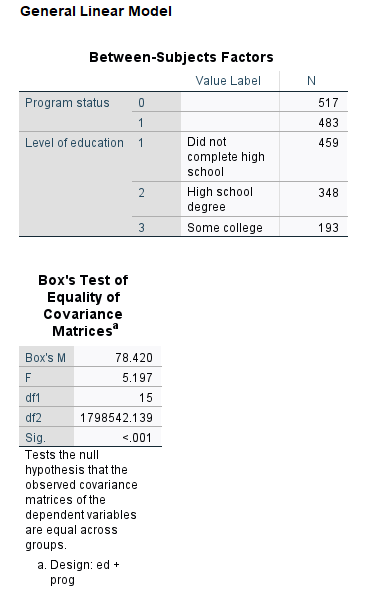
\includegraphics[width=0.5\linewidth]{Box's test} \newline
	
	\end{figure}
	
	\begin{figure}[h]
		
	
		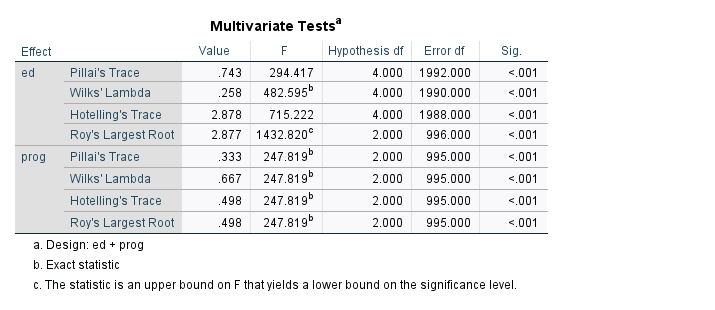
\includegraphics[width=1\linewidth]{Multivariate test}
	\end{figure}
	
		\begin{figure}[h]
		
		
		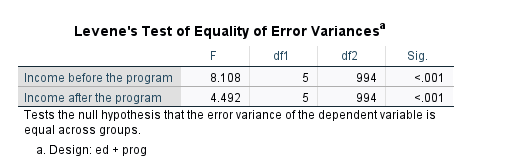
\includegraphics[width=1.5\linewidth]{Levene's test}
		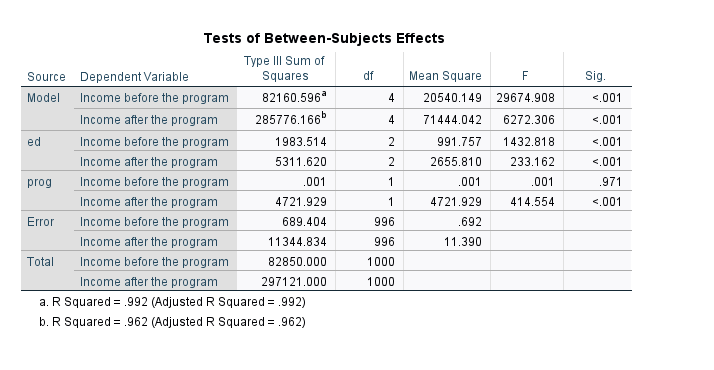
\includegraphics[width=1.5\linewidth]{Test between subject effect}
	\end{figure}

	\begin{figure}[h]	
	\subsection*{b.} Since the Box's Test of Equality of Covariance Matrices shows that we reject the null hypothesis (Sig. < 0.001), and conclude that homogeneity of covariance matrices is not met, it is necessary do the appropriate transformation(s) of the dependent variables.
	
	\subsubsection*{Log Transformation}
		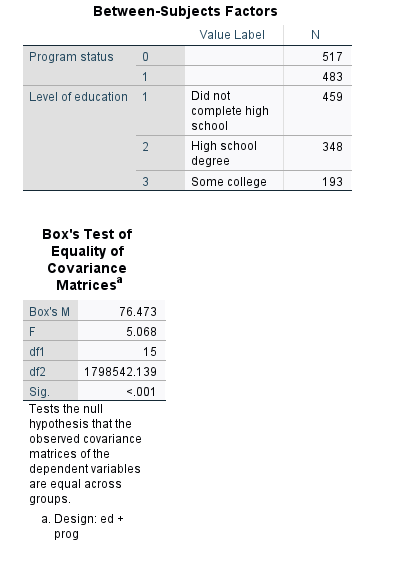
\includegraphics[width=0.8\linewidth]{Box's test1}
		
		
		\end{figure}
		
			\begin{figure}[h]
			
			
			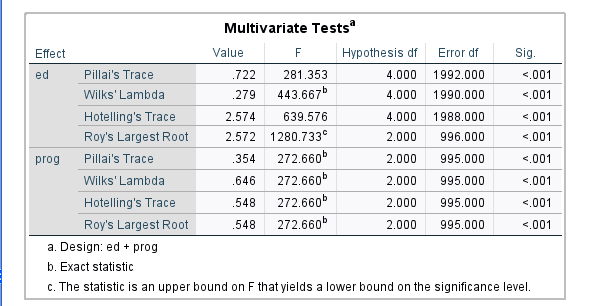
\includegraphics[width=1\linewidth]{Multivariate test1}
		\end{figure}
		
		\begin{figure}[h]
			
			
			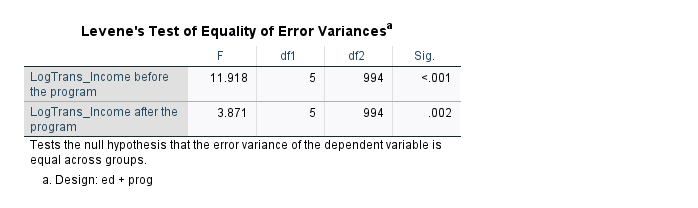
\includegraphics[width=1\linewidth]{Levene's test1}
			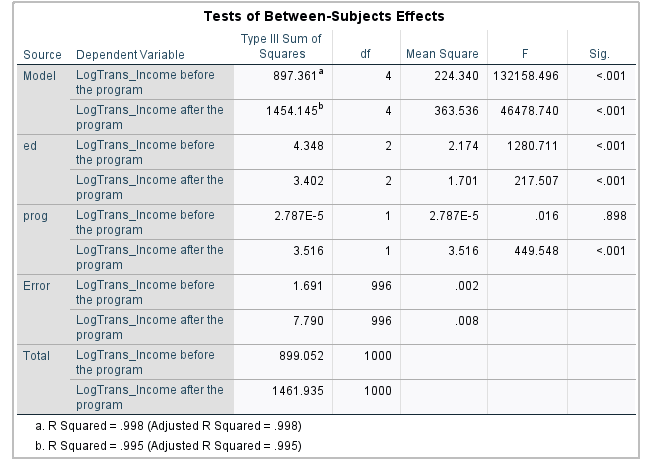
\includegraphics[width=1\linewidth]{Test between subject effect1}
		\end{figure}
		
			\begin{figure}[h]
			
			
			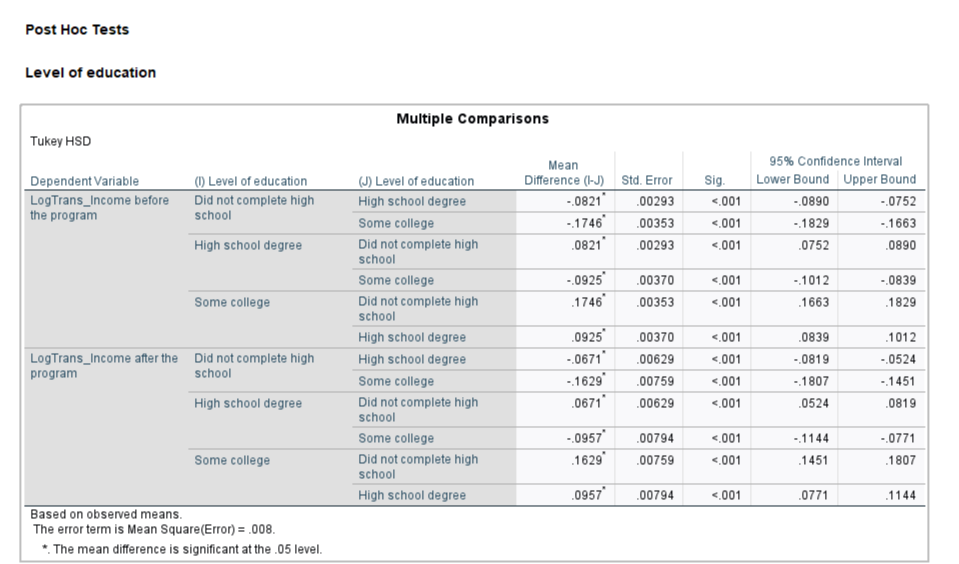
\includegraphics[width=1.2\linewidth]{Multiple comparisonLOG}
		\end{figure}
		
			
		
		
		
		\begin{figure}[h]
			
			
			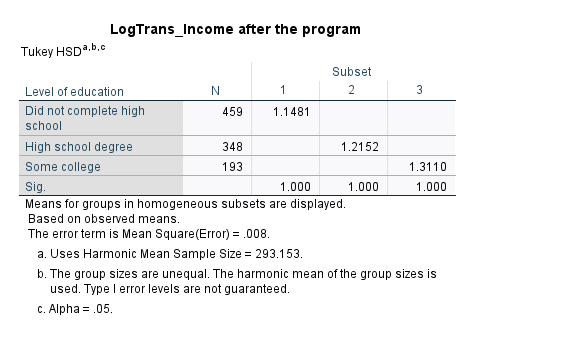
\includegraphics[width=1\linewidth]{IAPlog}
			
				\end{figure}
				
					\begin{figure}[h]
			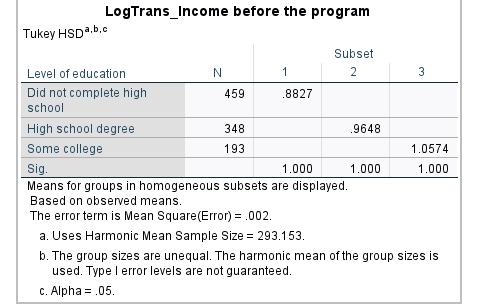
\includegraphics[width=1\linewidth]{IBPlog}
			
			\subsection*{c.}
			\subsubsection*{Box's Test of Equality of covarience matrices:}
			
			Observing the Box's Test of Equality of covarience matrices we notice the we notice that  though there is a decrease on the value of Box's M and its F-value, our results still indicate that homogeneity of covariance matrices is not met.
			
				\subsubsection*{Multivariate Tests:}
			Though there is a slight difference in the multivariate value, the result still remain significant(sig. <.001)
			
				\subsubsection*{Tests between subjects effects:}
			In observation of both not transformed and transformed data("Log-Trans Income before the program" and "LogTrans-Income after the program"), the p-values (Sig. column) are all less than 0.001, indicating that the between-subjects effects are statistically significant at the 0.001 level.The high F-statistics and low p-values suggest that the independent variables included in the model have a significant impact on the dependent variables thought there is a decrease in the p-value of a transformed "Income before the program" associate with "program status" and the Type III Sum of Squares have be transformed from larges values to small reasonable values though that does no change the results entirely
			
			\subsubsection*{In overall}
	Though results  of our analysis has changed the conclusion have not. Thefore the data violates homogeneity of covariance matrices.
			\end{figure}
%------------------------------------------------
			
		
	\begin{figure}[h]		
	\subsection*{d.}	
	
	\subsubsection*{Box's test}	
	Since the associated p-value for the Box’s M Test is <0.001, which is less than the desired significance level of 0.05, this suggests that homogeneity of covariances is not met
	
		\subsubsection*{Multivariate Tests:}
	For both the "educationa level" and "program status" independent variables, all the multivariate test statistics (Pillai's Trace, Wilks' Lambda, Hotelling's Trace, and Roy's Largest Root) have very low p-values (p < 0.001), indicating that the effects of these variables on the dependent variables are statistically significant.
	The high F-statistics and low p-values suggest that the independent variables included in the model have a significant impact on the overall set of dependent variables.
	
	\subsubsection*{Levene's Test of Equality of Error Variances.}
	For the "LogTrans-Income before the program" variable, the F-statistic is 11.918 with 5 and 994 degrees of freedom, and the p-value is less than 0.001.
	For the "LogTrans-Income after the program" variable, the F-statistic is 3.871 with 5 and 994 degrees of freedom, and the p-value is 0.002.
	The low p-values (less than 0.05) for both variables indicate that the we reject the null hypothesis of equal error variances across groups . In other words, the error variances are not equal across the groups defined by the independent variables(transformed Income
	before the program and Income after the program).
	
	\subsubsection*{Tests between subjects effects:}	
	For both "LogTrans-Income before the program" and "LogTrans-Income after the program", the p-values (Sig. column) are all less than 0.001, indicating that the between-subjects effects are statistically significant at the 0.001 level.The high F-statistics and low p-values suggest that the independent variables included in the model (" level od education" and "program status") have a significant impact on the dependent variables (LogTrans-Income before and after the program).
	
	\subsubsection*{post Hoc test:}
		The Tukey HSD test indicates that there are three homogeneous subsets (Subset 1, 2, and 3) for the "Level of education" variable.
	The "Did not complete high school" group has a mean of 7.6776, and it is in Subset 1, which is significantly different from the other two groups.
	The "High school degree" group has a mean of 9.2500, and it is in Subset 2, which is significantly different from the "Did not complete high school" group (Subset 1) but not significantly different from the "Some college" group (Subset 3).
	The "Some college" group has a mean of 11.4560, and it is in Subset 3, which is significantly different from the "Did not complete high school" group (Subset 1) but not significantly different from the "High school degree" group (Subset 2).
	
	
	For "Income before the program" the mean difference between "Did not complete high school" and "High school degree" is statistically significant (p < 0.001). The mean difference between "High school degree" and "Some college" is also statistically significant (p < 0.001). The mean difference between "Did not complete high school" and "Some college" is statistically significant (p < 0.001).
	
	For "Income after the program" the mean differences between all pairwise comparisons of the "Level of education" groups are statistically significant (p < 0.001).
	

	
	
		\end{figure}
		
	\begin{figure}[h]	
	\section*{Question 3 }
	\subsubsection*{(i)}
	
	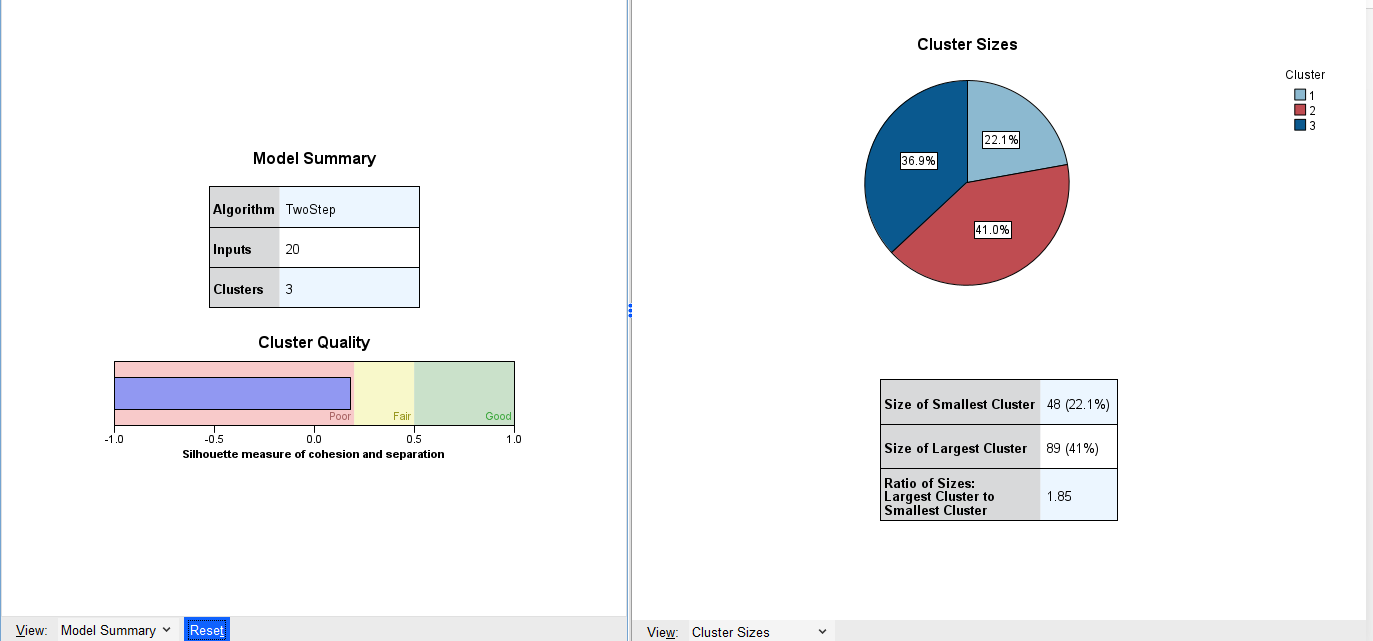
\includegraphics[width=1.3\linewidth]{Clusters}
	
	Number of Clusters: 3 clusters \newline
	Cluster Quality poor, based on the Silhouette measure.
\end{figure}

\begin{figure}[h]
	\subsubsection*{(ii)}
	
		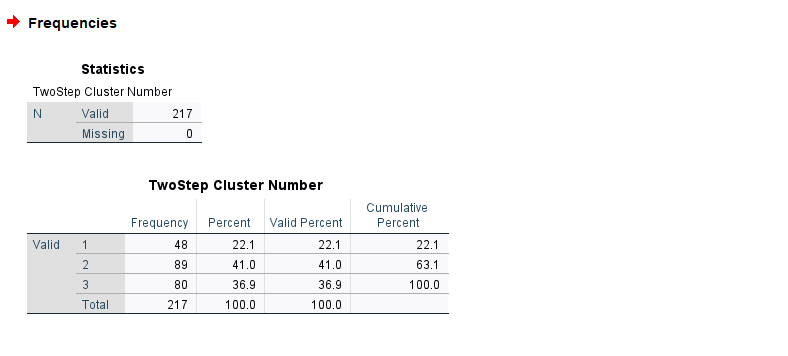
\includegraphics[width=1.5\linewidth]{cluster distribution of the cases1}
		
	Cluster Distribution: \newline
	Cluster 1: 48 cases (22.1\%) \newline
	Cluster 2: 89 cases (41.0\%) \newline
	Cluster 3: 80 cases (39.9\%) \newline
	\end{figure}
	 
			
		
	
\end{document}	